\documentclass{article}
\usepackage{graphicx}
\usepackage{float}
\usepackage{amsmath}
\usepackage{amssymb}

\usepackage[french]{babel}
\usepackage[utf8]{inputenc}

%%%%%%%%%%%%%%%% Lengths %%%%%%%%%%%%%%%%
\setlength{\textwidth}{15.5cm}
\setlength{\evensidemargin}{0.5cm}
\setlength{\oddsidemargin}{0.5cm}

%%%%%%%%%%%%%%%% Variables %%%%%%%%%%%%%%%%
\def\projet{2}
\def\titre{Résolution de systèmes linéaires / Application à l’équation de la chaleur}
\def\groupe{2}
\def\equipe{2}
\def\responsible{Yani Haouchine}
\def\secretary{Arnaud Chane-Kive}
\def\others{Wissal Faouzi, Vivien Nebout}

\begin{document}

%%%%%%%%%%%%%%%% Header %%%%%%%%%%%%%%%%
\noindent\begin{minipage}{0.98\textwidth}
  \vskip 0mm
  \noindent
  { \begin{tabular}{p{7.5cm}}
      {\bfseries \sffamily
        Projet \projet} \\ 
      {\itshape \titre}
    \end{tabular}}
  \hfill 
  \fbox{\begin{tabular}{l}
      {~\hfill \bfseries \sffamily Groupe \groupe\ - Equipe \equipe
        \hfill~} \\[2mm] 
      Responsable : \responsible \\
      Secrétaire : \secretary \\
      Codeurs : \others
    \end{tabular}}
  \vskip 4mm ~

  ~~~\parbox{0.95\textwidth}{\small \textit{Résumé~:} \sffamily Ce projet a pour but d'implémenter des algorithmes de résolution de systèmes linéaires de grande taille, puis de les appliquer à l'équation de la chaleur. Dans la première partie, nous parlerons de la méthode directe avec la méthode de Cholesky, puis dans la seconde partie de la méthode itérative avec la méthode du gradient conjugué, et enfin la méthode itérative préconditionnée avec la méthode de Cholesky incomplète.}
  \vskip 1mm ~
\end{minipage}

%%%%%%%%%%%%%%%% Main part %%%%%%%%%%%%%%%%
\section*{Résolution de système linéaire}

Pour résoudre un système linéaire de la forme suivante :
\[
\begin{bmatrix}
a_{11} & a_{12} & \dots & a_{1n} \\
a_{21} & a_{22} & \dots & a_{2n} \\
\vdots & \vdots & \ddots & \vdots \\
a_{m1} & a_{m2} & \dots & a_{mn}
\end{bmatrix}
\begin{bmatrix}
x_1 \\ x_2 \\ \vdots \\ x_n
\end{bmatrix}
=
\begin{bmatrix}
b_1 \\ b_2 \\ \vdots \\ b_m
\end{bmatrix}
\]

il existe deux familles de méthodes; les méthodes itératives, et les méthodes directes.
Les méthodes directes consistent à trouver une solution exacte (en théorie) en un nombre borné d'opérations. Bien que ce nombre soit borné, il est souvent en pratique trop grand. 
Les méthodes itératives, elles, consistent à trouver une suite de vecteurs convergeant vers la solution exacte avec un coût en mémoires souvent plus bas que les méthodes directes. Ces méthodes ne convergent pas toujours et nécessitent parfois des préconditionnements pour améliorer leur efficacité.
Tout au long du rapport, n sera le rang de A.
\subsection*{Méthode direct}
La méthode directe qui nous est proposée d'implémenter est la méthode de Cholesky, à l'aide de cette méthode, la résolution de notre système linéaire se fait en O(n³).
\subsubsection{Conception}
La méthode de Cholesky consiste à factoriser une matrice symétrique définie positive A en un produit d'une matrice triangulaire et de sa transposée. Pour tout système triangulaire se résolvant "rapidement", on comprend l’intérêt d'une telle décomposition.
\subsubsection*{Implémentation}
Notre implémentation essaie de se rapprocher le plus possible de l'algorithme présenté en cours. On y retrouve la construction d'une nouvelle matrice triangulaire T; le parcours de ces éléments en suivant les lignes et les colonnes, et la disjonction de cas suivant que l'on calcule un élément diagonal ou non.
Cette proximité, bien que facilitant la compréhension de notre algorithme, a un coût en ressources.
Par exemple, on ne cherche pas à reconnaître des produits scalaires, pouvant, avec l'utilisation de np.dot, faire profit du parallélisme et donc réduire le temps de calcul.
On ne cherche aussi pas à stocker T dans A, ce qui aurait pu améliorer notre complexité en espace.
\subsubsection*{Complexité}
La complexité de notre algorithme vient du fait que pour chaque élément de T, il faille calculer une somme possiblement de n - 1 éléments.
Il y a \( \Theta \)(n²) éléments à calculer dans T, cet algorithme s’exécute donc en \( \Theta \)(n³) opérations.

\subsection*{Méthode itérative}
La méthode itérative qu'il nous est proposé d'effectuer est la méthode du gradient conjugué. 
\subsubsection*{Implémentation}
Pour implémenter cet algorithme, on se base sur le code Matlab fourni. Seulement certains points ont dû être corrigés, comme la précision qui était beaucoup trop élevée, et le fait que l'algorithme proposé ne renvoie rien. 
\subsubsection*{Complexité et convergence}
Comme cela a été vu en cours, la complexité et la convergence de cet algorithme dépendent directement du conditionnement de notre entrée et d'à quel point la matrice est creuse.
Ainsi, si le nombre d'éléments non nuls de la matrice est un O(n) alors notre algorithme s'exécutera en \( \Theta \)(n²).
\subsection*{Méthode itérative préconditionnée}
Comme énoncée ci-dessus, la qualité de notre algorithme dépend entièrement de notre entrée. Afin de profiter de cette remarque nous nous proposons donc de préconditionner notre matrice avant de la passer en argument à notre algorithme itératif.
\subsubsection*{Méthode Cholesky incomplète}
Pour préconditionner notre matrice, nous choisissons d'utiliser la méthode de Cholesky incomplète.
Pour une matrice n'ayant aucune valeur nulle, cette méthode est équivalente à la méthode de Cholesky classique. Pour les matrices creuses néanmoins, cet algorithme devient particulièrement efficace. Plus généralement, comme cet algorithme ne calcule pas les valeurs tij pour lesquelles aij sont nuls. Si on appelle m le nombre de valeurs non nulles de notre matrice A, on a comme complexité pour Cholesky incomplet O(n*m).
Pour tester cette méthode, il nous faut donc pouvoir construire des matrices creuses symétriques définies positives, ce qui sera explicité dans la sous-section prochaine.
\subsubsection*{Matrices creuses}
L'idée ici est de s'appuyer sur le fait que toutes les matrices à diagonales strictement dominantes sont définies positives.
Supposant que l'on veuille construire une matrice A symétrique définie positive ayant m coefficients extra-diagonaux non nuls, (m est pair puisque A est triangulaire), on procède comme suit.
On construit une matrice L triangulaire inférieure stricte dont on choisit aléatoirement la position de m/2 éléments non nuls. On additionne L et sa transposée puis on choisit ces coefficients diagonaux de façons à ce que :\( A = (a_{ij}) \in \mathbb{R}^{n \times n} \) on ait pour tout \( i \in \{1, \dots, n\} \),
\[
|a_{ii}| > \sum_{\substack{j=1 \\ j \neq i}}^{n} |a_{ij}|.
\]
 ainsi la matrice est diagonale dominante, et donc définie positive et symétrique et possède seulement m coefficients non nuls.
\subsubsection*{Efficacité comparé à la méthode de Cholesky}
Nous n'avons pas eu le temps d'implémenter complètement une méthode itérative préconditionnée, seulement, d'après les résultats établit en cours, cette méthode diminuerai le nombre d'itération requis à la convergence.
\subsection*{Résolution de l'équation de la chaleur}
Nous nous proposons dans cette partie de résoudre l'équation de la chaleur.
\subsubsection{Intêret}
En supposant que les équations et les algorithmes proposés soient corrects, essayer de résoudre les équations de la chaleur est une bonne façon de vérifier la validité de notre implémentation.
En effet, nous avons tous une idée plus ou moins exacte de la façon dont la température se répartit dans une salle, en présence d'une source de chaleur.
Ainsi, simuler et représenter cette répartition, est donc un moyen visuel, rapide, intuitif et plus ou moins efficace de vérifier la validité de notre implémentation.
\subsubsection*{Conception}
On représente notre problème sous forme matricielle, le vecteur x sera l'ensemble des points dont on voudra calculer la température, le vecteur b sera la source de température et la matrice A représentera la façon dont les points contigus s'influencent entre eux.
On résout ensuite ce système, à l'aide des deux méthodes présentées plus haut.

\newpage

\subsubsection*{Résolution à l'aide de méthode directe}
Voici les différentes figures obtenues à l'aide d'une méthode de Cholesky :





\begin{figure}[H]
    \centering
    \begin{minipage}{0.49\linewidth}
        \centering
        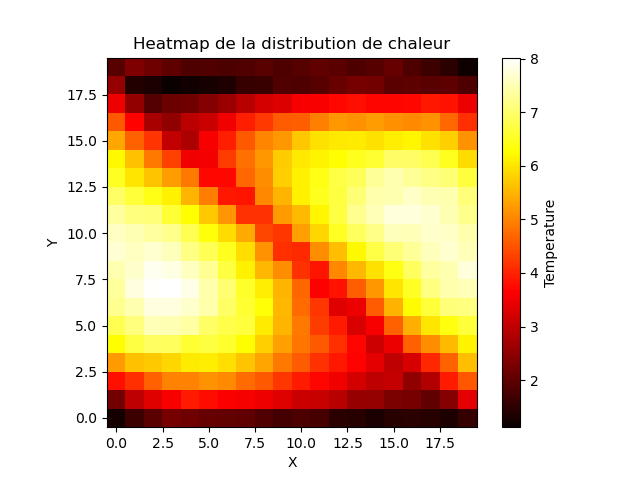
\includegraphics[width=\linewidth]{Figure_3.png}
        \caption{Test avec source de chaleur aléatoire et méthode itérative}
        \label{fig:1}
    \end{minipage}
    \hfill
    \begin{minipage}{0.49\linewidth}
        \centering
        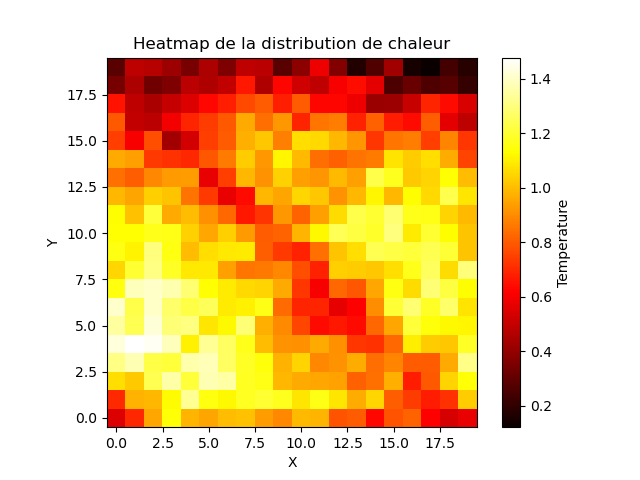
\includegraphics[width=\linewidth]{Figure_4.png}
        \caption{Test avec source de chaleur aléatoire et méthode directe}
        \label{fig:2}
    \end{minipage}
\end{figure}





\begin{figure}[H]
    \centering
    \begin{minipage}{0.49\linewidth}
        \centering
        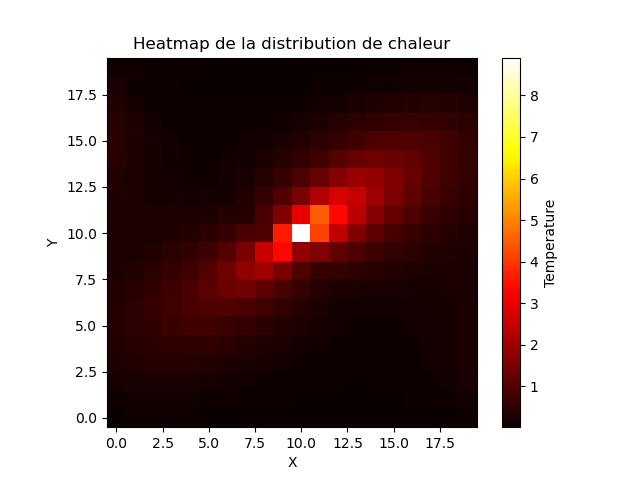
\includegraphics[width=\linewidth]{Figure_5.png}
        \caption{Test avec source de chaleur au centre et méthode itérative}
        \label{fig:3}
    \end{minipage}
    \hfill
    \begin{minipage}{0.49\linewidth}
        \centering
        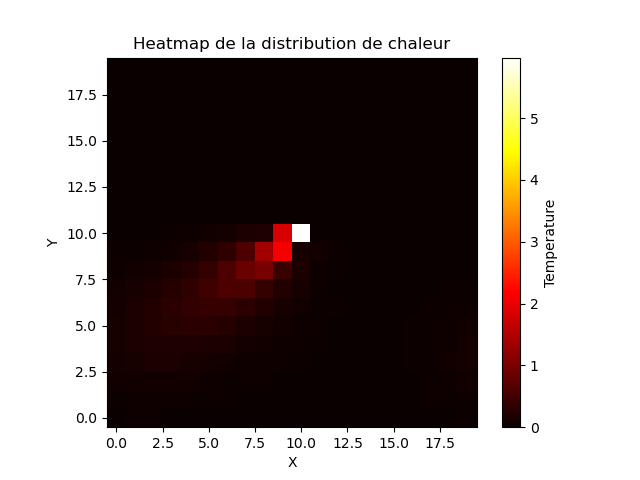
\includegraphics[width=\linewidth]{Figure_6.png}
        \caption{Test avec source de chaleur au centre et méthode directe}
        \label{fig:4}
    \end{minipage}
\end{figure}



\newpage

\subsubsection*{Interprétation}
La chaleur se répartissant de la même façon selon toutes les directions, les asymétries aux niveaux des figures ci-dessus nous portent à croire que notre implémentation est inefficace.
En particulier, la figure\label{3} et la figure\label{4} sont censé représenter des répartitions où la source est placée au milieu de la grille. On voit que la répartition de la chaleur a une direction privilégiée, ce qui n'est pas cohérent avec les observations réelles.

\section*{Conclusion}
En conclusion, bien que partiellement, nous avons appris à implémenter des méthodes de résolution de systèmes linéaires et à appliquer ces méthodes pour la résolution de problèmes réels comme l'équation de la chaleur.


\end{document}

